\subsection{Schnyder-Wood-Fluss}

Um einen Schnyder Wood als Fluss-Problem zu kodieren, kann man die in Abschnitt \ref{alpha_orientations} eingeführten $\alpha_s$-Orientierungen auf dem Abschluss von $G+G^*$ nutzen. Fusy zeigt in \cite{fusy07} im Zuge der Untersuchung spezifischer $\alpha$-Funktionen, dass sich $\alpha_s$-Orientierungen von $G+G^*$ in linearer Zeit berechnen lassen, sodass wir auch einen Schnyder Wood auf $G$ in linearer Zeit erhalten.

Sei ein ebener intern-3-zusammenhängender Graph $G$ mit Aufhängungen $a_1,a_2,a_3$ gegeben. Machen wir uns an die Konstruktion eines Netzwerks $\mathcal{N}_S$, sodass ein zulässiger ganzzahliger Fluss $\varphi_s$ auf $\mathcal{N}_S$ einer $\alpha_s$-Orientierung von $G+G^*$ entspricht\footnote{Hier stehen die drei \textit{s} jeweils für Schnyder um spätere Verwechslungen zu vermeiden.}. Nach Theorem \ref{alpha_bij} würde die aus $\varphi_s$ erhaltene $\alpha_s$-Orientierung somit auch einen Schnyder Wood auf $G$ induzieren. Besonderes Augenmerk ist hier auf die Möglichkeit einer späteren Kombination mit einem weiteren Netzwerk gelegt, in welchem eine ganzzahlige Lösung einem FAA auf $G$ entspricht, um ein kombiniertes Netzwerk zu erstellen.

Wie schon erwähnt ist $G+G^*$ bipartit, Kanten-Knoten haben Grad 4, Knoten-Knoten haben Grad $\text{deg}(v)$ und Gebiets-Knoten haben Grad $|f|$. Für eine $\alpha_s$-Orientierung muss nach Definition \ref{alpha_bij} A3 jeder Kanten-Knoten Ausgangsgrad 1, jeder Knoten-Knoten Eingangsgrad $\text{deg}(v)-3$ und jeder Gebiets-Knoten Eingangsgrad $|f|-3$ haben. Die Kanten-Knoten am äußeren Gebiet sind in $G+G^*$ immer nach außen orientiert. Somit reicht es, wenn wir nur die inneren Kanten-Kanten $E_{in}$ betrachten und die Orientierung der äußeren Kanten voraussetzten.

\begin{figure}[h]
	\centering
  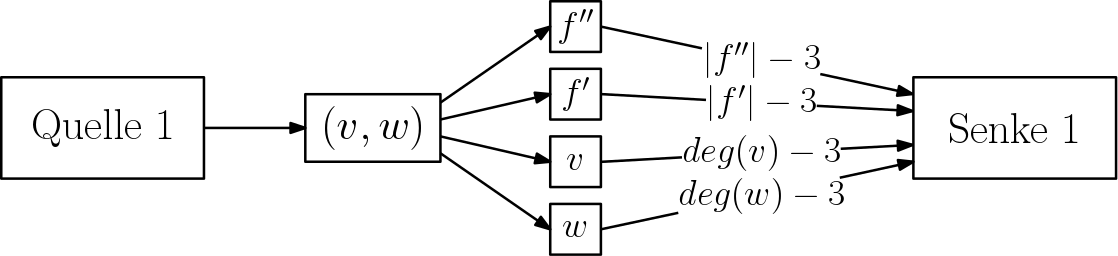
\includegraphics[width=0.9\textwidth]{schnyder_flow.png}
  \caption{Der Schnyder Wood Fluss durch eine innere Kante $(v,w)$. Die nicht beschrifteten Kanten haben Kapazität 1.}
  \label{schnyder_flow}
\end{figure}

Das im Folgenden konstruierte Netzwerk ist in Abbildung \ref{schnyder_flow} skizziert und unter dem Punkt Netzwerk \ref{net_schnyder} zusammengefasst. Das Netzwerk $\mathcal{N}_S$ hat eine Quelle $s$ und eine Senke $t$ und einen Knoten für jeden Knoten aus $G+G^*$ (bis auf die äußeren Kanten). Es existieren Kanten von der Quelle zu jedem Kanten-Knoten $e \in E_{in}$ mit Kapazität 1. Von den Kanten-Knoten $e$ zu inzidenten Knoten-Knoten $v$ und Gebiets-Knoten $f \in F_{in}$ fügen wir ebenfalls Kanten mit Kapazität 1 ein. Merke, dass der Fluss auf diesen Kanten bei einer ganzzahligen Lösung eine $\alpha_s$-Orientierung auf $G+G^*$ ergeben soll. Nun fügen wir noch Kanten von $f \in F_{in}$ zur Senke mit Kapazitäten $|f|-3$, Kanten von den (inneren) Knoten-Knoten $v \in V_{in} = V \setminus \{a_1,a_2,a_3\}$ zur Senke mit Kapazitäten $\text{deg}(v)-3$ und Kanten von den Aufhängungen $a_i$ zur Senke mit Kapazitäten $\text{deg}(a_i)-2$. Die letzte Kapazität ergibt sich, da die Halbkante in $G+G^*$ von $a_i$ aus immer nach außen orientiert. Wir müssen somit nur noch zwei andere Kanten von $a_i$ weg orientieren. Der Bedarf des Netzwerkes entspricht der Anzahl der inneren Kanten von $G$. Fassen wir zusammen.

\begin{network}[Schnyder Wood]\label{net_schnyder}
Bei $\mathcal{N}_S$ handelt es sich um ein gerichtetes Netzwerk, das auf Basis eines ebenen intern-3-zusammenhängenden Graphen $G$ mit Aufhängungen $a_1,a_2,a_3$ erstellt wird, um einen Schnyder Wood auf $G$ zu finden. Ein Ausschnitt ist in Abbildung \ref{schnyder_flow} dargestellt.
	\begin{itemize}
	\item $\mathcal{N}_S$ hat eine Quelle $s$ und eine Senke $t$
	\item Knoten in $\mathcal{N}_S$ werden für jeden innere Kante $e \in E_{in}$, jedes innere Gebiet $f\in F_{in}$ und jeden Knoten $v \in V$ aus $G$ erzeugt.
	\item Es werden gerichtete Kanten der folgenden Typen in $\mathcal{N}_S$ erzeugt:
		\begin{itemize}
		\item $(s,e)$ von der Quelle zu jeder inneren Kante mit $c\big(s,e\big) = 1$
		\item $(e,v_1),(e,v_2)$ von jeder inneren Kante zu den Endknoten mit $c\big(e,v\big) = 1$
		\item $(e,f)$ von jeder inneren Kante zu adjazenten Gebieten mit $c\big(e,f\big) = 1$
		\item $(v,t)$ von den Knoten zur Senke mit $c\big(v,t\big) = 1$
		\item $(f,t)$ von den inneren Gebieten zur Senke mit $c\big(f,t\big) = |f|-3$
		\item $(a_i,t)$ von den Aufhängungen zur Senke mit $c\big(f,t\big) = \text{deg}(a_i)-2$
		\item $(v,t)$ von den restlichen Knoten zur Senke mit $c\big(f,t\big) = \text{deg}(v)-3$
		\end{itemize}
	\item $\mathcal{N}_S$ hat Bedarf $d=|E_{in}|$
	\item [$\Rightarrow$] Ein zulässiger ganzzahliger Fluss $\varphi_s$ existiert genau dann, wenn ein Schnyder Wood  auf $G$ existiert.
	\end{itemize}
\end{network}

\begin{proposition}
Sei $G$ ein ebener intern-3-zusammenhängender Graph mit Aufhängungen $a_1,a_2,a_3$ und $\mathcal{N}_S$ wie in Netzwerk \ref{net_schnyder} konstruiert. Ein ein zulässiger ganzzahliger Fluss $\varphi_s$ auf $\mathcal{N}_S$ existiert genau dann, wenn ein Schnyder Wood auf $G$ zu den Aufhängungen $a_1,a_2,a_3$ existiert. Insbesondere kodiert jeder Fluss einen Schnyder Wood.
\end{proposition}

\begin{proof}
Sei $\varphi_s$ ein zulässiger ganzzahliger Fluss auf $\mathcal{N}_S$. Es gilt $|\varphi_s| = |E_{in}|$. Somit hat jede innere Kante-Knoten Ausgangsgrad 1. Weiter gilt 
$$\sum_{v \in V} \Big(\text{deg}(v)-3\Big) + 3 + \sum_{f \in F_{in}} \Big(|f|-3\Big) = |E_{in}|.$$
Somit sind die Kanten von den Kanten-Knoten und Knoten-Knoten ausgelastet. Der Fluss $\varphi_s$ entlang einer Auskante von $e \in E_{in}$ in $\mathcal{N}_S$ entspricht dann genau der Kante in $G+G^*$, die in der $\alpha_{s}$-Orientierung von $e$ weg orientiert wird. Durch die Knoten-Knoten $v$ und Gebiets-Knoten $f$ fließt Fluss auf $\text{deg}(v)-3$ bzw. $|f|-3$ Kanten der von den Kanten-Knoten kommt. Somit lässt $\varphi_s$ jeweils drei Kanten frei, denen wir noch keine Orientierung zugewiesen haben. Diese entsprechen somit den von $v$ bzw. $f$ weg orientierten Kanten einer $\alpha_{s}$-Orientierung auf $G+G^*$. Somit hat jedes Gebiet und jeder Knoten den passenden Ausgangsgrad und $\varphi_s$ kodiert eine $\alpha_s$-Orientierung auf $G+G^*$. Auf analoge Weise lässt sich aus einer $\alpha_s$-Orientierung ein zulässiger ganzzahliger Fluss $\varphi_s$ erstellen. Es existiert also genau dann ein Schnyder Wood auf $G$, wenn eine ganzzahlige Lösung $\varphi_s$ für $\mathcal{N}_S$ existiert.
\end{proof}

\subsection{FAA-Fluss}\label{faa-flow}

Sei wieder ein ebener intern-3-zusammenhängender Graph $G$ mit Aufhängungen $a_1,a_2,a_3$ gegeben. Ein FAA ordnet nun jedem Gebiet $|f|-3$ flache Winkel zu und jeder Knoten darf maximal einem Gebiet zugeordnet werden. Die adjazenten Knoten um das äußere Gebiet, die keine Aufhängungen sind, müssen diesem zugewiesen werden. Wir konstruieren ein Netzwerk $\mathcal{N}_F$, für das ein ganzzahliger zulässiger Fluss einem FAA entspricht 

\begin{figure}
	\centering
  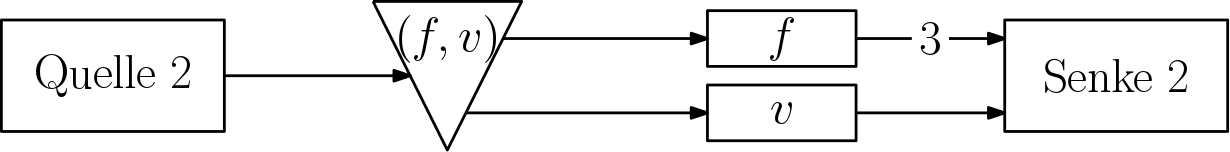
\includegraphics[width=0.8\textwidth]{faa_flow.png}
  \caption{Der FAA-Fluss durch einen Winkel $(f,v)$. Die nicht beschrifteten Kanten haben Kapazität 1.}
  \label{faa_flow}
\end{figure}

Das im Folgenden konstruierte Netzwerk ist in Abbildung \ref{faa_flow} skizziert und unter dem Punkt Netzwerk \ref{net_faa} zusammengefasst. Das Netzwerk $\mathcal{N}_F$ hat jeweils eine Quelle und Senke. Wir erstellen in $\mathcal{N}_F$ Knoten für jeden inneren Winkel $(f,v)$, mit $v\in V$ und $f \in F_{in}$, Knoten für alle inneren Gebiete $f \in F_{in}$ und für die inneren Knoten $v\in V_{in}$. Von der Quelle fügen wir Kanten mit Kapazität 1 zu jedem inneren Winkel $(f,v)$, und von jedem inneren Winkel $(f,v)$ jeweils eine Kante zu $f$ und zu $v$ (falls $v\in V_{in}$) mit Kapazität 1 ein. Merke, dass so der Fluss von den Winkeln zu den inneren Knoten einem FAA entspricht. Zuletzt erstellen wir Kanten von jedem inneren Gebiet $f$ zur Senke mit Kapazität 3 und Kanten von jedem Knoten $v$ zur Senke mit Kapazität 1 ein. Der Bedarf des Netzwerks ist $\sum_{f \in F_{in}}|f|$ und entspricht der Anzahl der inneren Winkel von $G$. Fassen wir zusammen.

\begin{network}[FAA]\label{net_faa}
Bei $\mathcal{N}_F$ handelt es sich um ein gerichtetes Netzwerk, das auf Basis eines ebenen intern-3-zusammenhängenden Graphen $G$ mit Aufhängungen $a_1,a_2,a_3$ erstellt wird, um ein FAA zu finden. Ein Ausschnitt ist in Abbildung \ref{faa_flow} dargestellt.
	\begin{itemize}
	\item $\mathcal{N}_F$ hat eine Quelle $s$ und eine Senke $t$
	\item Knoten in $\mathcal{N}_F$ werden für jeden inneren Winkel $(f,v) \in W_{in}$, jedes innere Gebiet $f\in F_{in}$ und jeden Knoten $v \in V$ aus $G$ erzeugt.
	\item Es werden gerichtete Kanten der folgenden Typen in $\mathcal{N}_F$ erzeugt:
		\begin{itemize}
		\item $(s,(f,v))$ von der Quelle zu jedem inneren Winkel mit $c\big(s,(f,v)\big) = 1$
		\item $((f,v),v)$ von jedem inneren Winkel zum Knoten mit $c\big((f,v),v\big) = 1$
		\item $((f,v),f)$ von jedem inneren Winkel zum Gebiet mit $c\big((f,v),f\big) = 1$
		\item $(f,t)$ von den inneren Gebieten zur Senke mit $c\big(f,t\big) = 3$
		\item $(v,t)$ von den Knoten zur Senke mit $c\big(f,t\big) = 1$
		\end{itemize}
	\item $\mathcal{N}_F$ hat Bedarf $d=\sum_{f \in F_{in}}|f|$
	\item [$\Rightarrow$]Ein zulässiger ganzzahliger Fluss $\varphi_F$ existiert genau dann, wenn ein FAA existiert.
	\end{itemize}
\end{network}

\begin{proposition}\label{prop_net_faa}
Sei $G$ ein ebener intern-3-zusammenhängender Graph mit Aufhängungen $a_1,a_2,a_3$ und $\mathcal{N}_F$ wie in Netzwerk \ref{net_faa} konstruiert. Ein ein zulässiger ganzzahliger Fluss $\varphi_F$ auf $\mathcal{N}_S$ existiert genau dann, wenn ein FAA auf $G$ zu den Aufhängungen $a_1,a_2,a_3$ existiert. Insbesondere kodiert jeder Fluss genau ein FAA.
\end{proposition}

\begin{proof}
Sei $\varphi_F$ ein zulässiger ganzzahliger Fluss auf $\mathcal{N}_F$. Der Fluss auf einer Kante $((f,v),f)$ entspricht einer Ecke von $f$ und Fluss auf $((f,v),u)$ der Zuweisung eines Knoten zu $f$. Zur Vereinfachung sprechen wir im Weitern auch von Ecken- und Zuweisungs-Fluss. Somit wird jeder innere Winkel von $\varphi_F$ entweder einem Gebiet zugewiesen oder als Ecke ausgezeichnet. Da die Kanten von den inneren Knoten zur Senke Kapazität eins haben kann jeder Knoten nur einmal zugewiesen werden. F2 ist somit erfüllt. Von jedem inneren Gebiet $f$ fließt Fluss mir Stärke $|\varphi_s(f,t)| = 3$ zu Senke. Somit muss $|f|-3$ Fluss durch zugewiesene Knoten gehen. F1 ist somit erfüllt. $\varphi_F$ respektiert also die Bedingungen aus Definition \ref{def_faa} und es existieren nur dann FAAs auf $G$, wenn mindestens eine ganzzahlige Lösung für $\mathcal{N}_F$ existiert.
\end{proof}

\begin{remark}

Das oben eingeführte Netzwerk \ref{net_faa} zur Bestimmung von FAAs lässt sich auch als Zwei-Fluss-Problem konstruieren. Wir trennen für Ecken- und Zuweisungs-Fluss die Quellen und Senken.  Zu jedem Winkelknoten $(f,v)$ fügen wir eine Kopie $(f,v)'$ ein und verbinden beide durch eine Kante mit Kapazität 1 (siehe Abbildung \ref{faa_as_2}). In den ersten führt eine Kante von beiden Quellen mit Kapazität 1. Und vom zweiten aus führen Kanten zu $f$ und $v$. Der Bedarf des Ecken-Flusses ist dann $3|F_{in}|$ und der Bedarf des Zuweisung-Flusses $\sum_{f \in F_{in}}{|f|-3}$.

\begin{figure}[h]
	\centering
  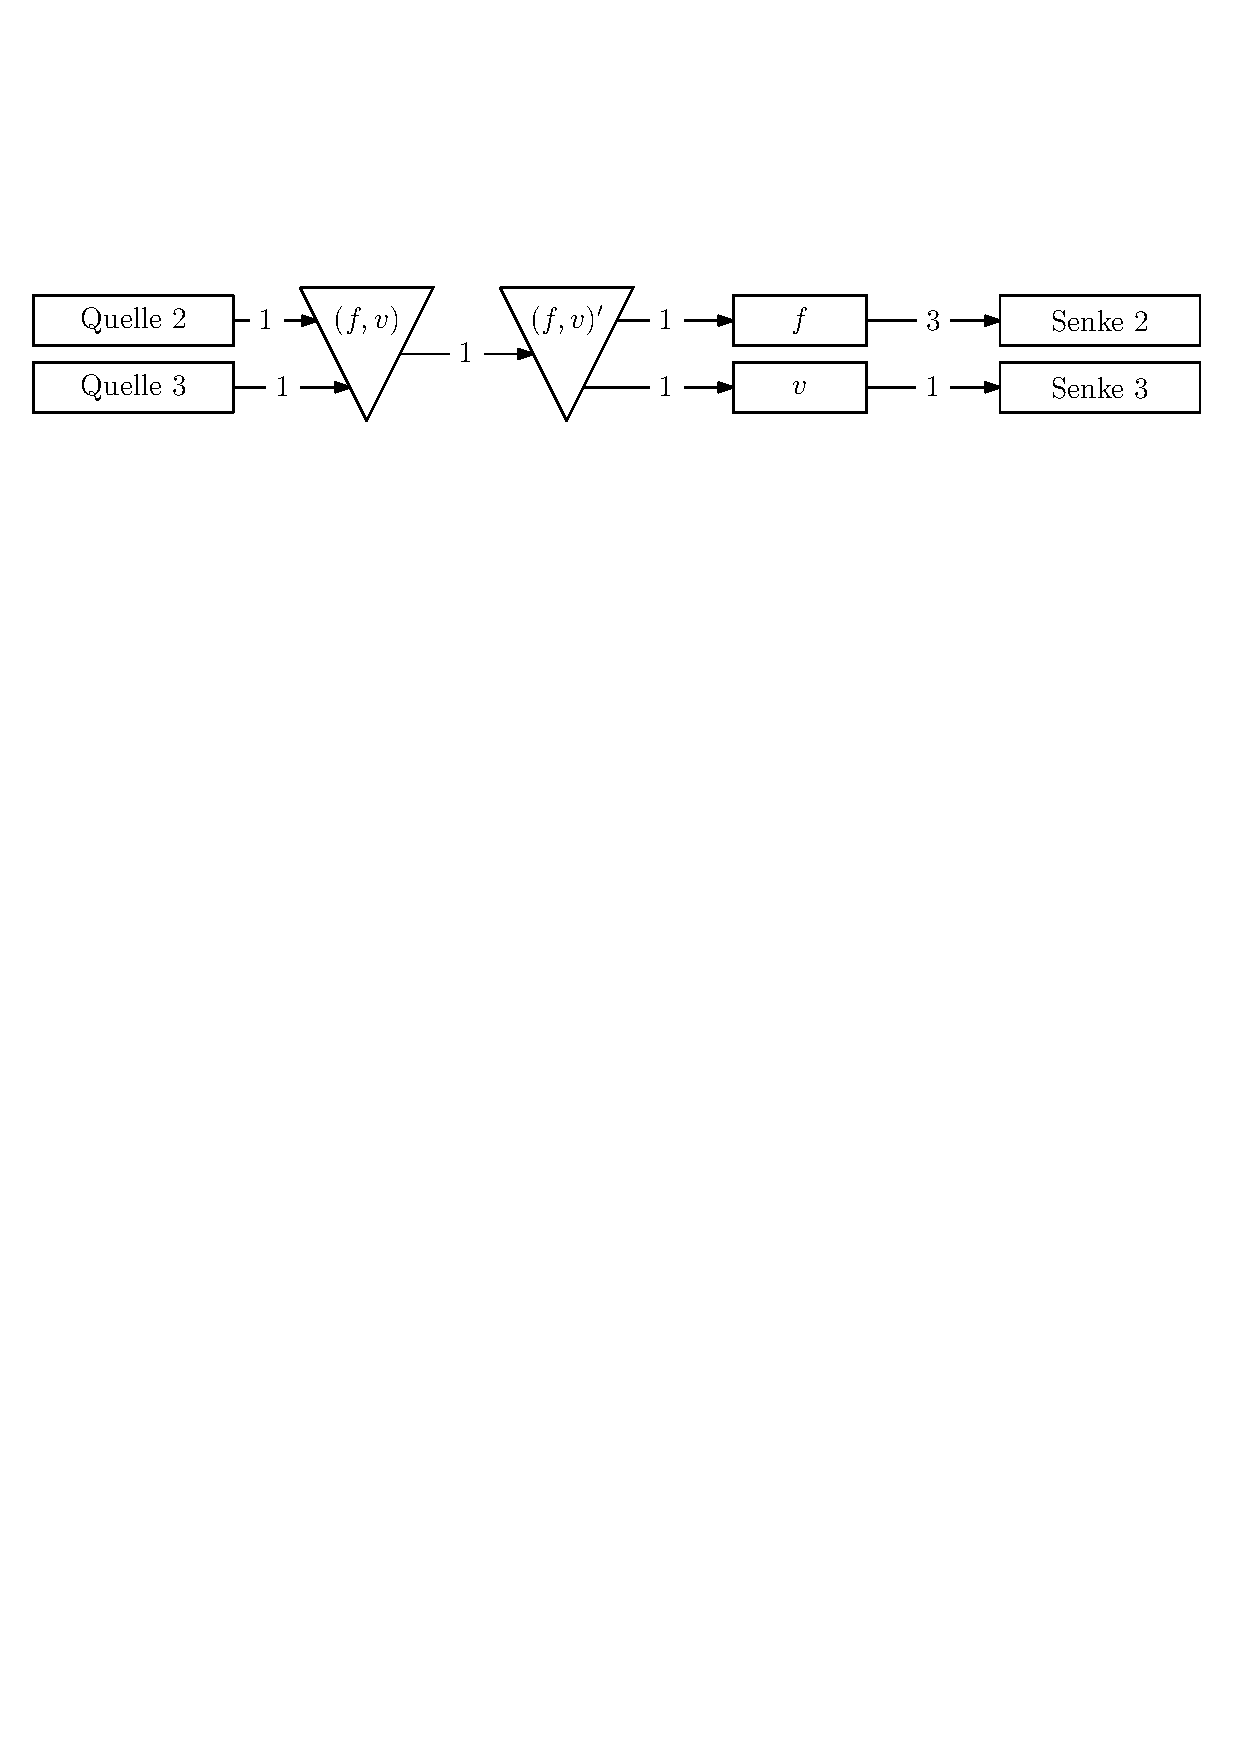
\includegraphics[width=0.8\textwidth]{faa_2_flow.pdf}
  \caption{Das einfügen einer Kante und eines zweiten Winkel Knotens gewährt die Trennung von Winkel- und Zuweisungs-Fluss. Die nicht beschrifteten Kanten haben Kapazität 1.}
  \label{faa_as_2}
\end{figure}

Eine zulässige ganzzahlige Lösung $\varphi_F = (\varphi_e,\varphi_z)$ entspricht dann wieder einem FAA auf $G$. Aus der Ganzzahligkeit folgt, dass ein Winkel entweder von $\varphi_{e}$ (Ecke) oder $\varphi_{z}$ (Zuweisung) genutzt wird. Dies gewährleisten die Kanten zwischen den Winkelknoten, da sie immer nur von einem der beiden Flüssen genutzt werden können.
\end{remark}


